\documentclass[prd,aps,twocolumn,a4paper,showkeys,nofootinbib]{revtex4-2}

\usepackage{amsmath}
\usepackage{amsfonts}
\usepackage{amssymb}	
\usepackage{graphicx}
\usepackage{color}
\usepackage[hidelinks]{hyperref}
\allowdisplaybreaks

\def\TODO{\textcolor{red}{TODO:}}
\def\Mc{{\cal M}_c}

\begin{document}

\title{Classification of NS data}

\author{Marina Berbel}

\date{\today}

\maketitle

%==========================================================
\section{Random forest}
%==========================================================


\subsection{Using only independent recovered variables}
Training and testing using: $m1_{rec}, m2_{rec}, chi1_{rec}, chi2_{rec}, snr$.
Standard deviation of score during crossvalidation:  0.000277942225285724 . Mean:  0.9744487408123469
Score  0.9748495808263471 . Optimum forest found:  200  trees,  entropy  criteria and  sqrt  max features

Score on testing:  0.9747829130485508

\begin{figure}[]
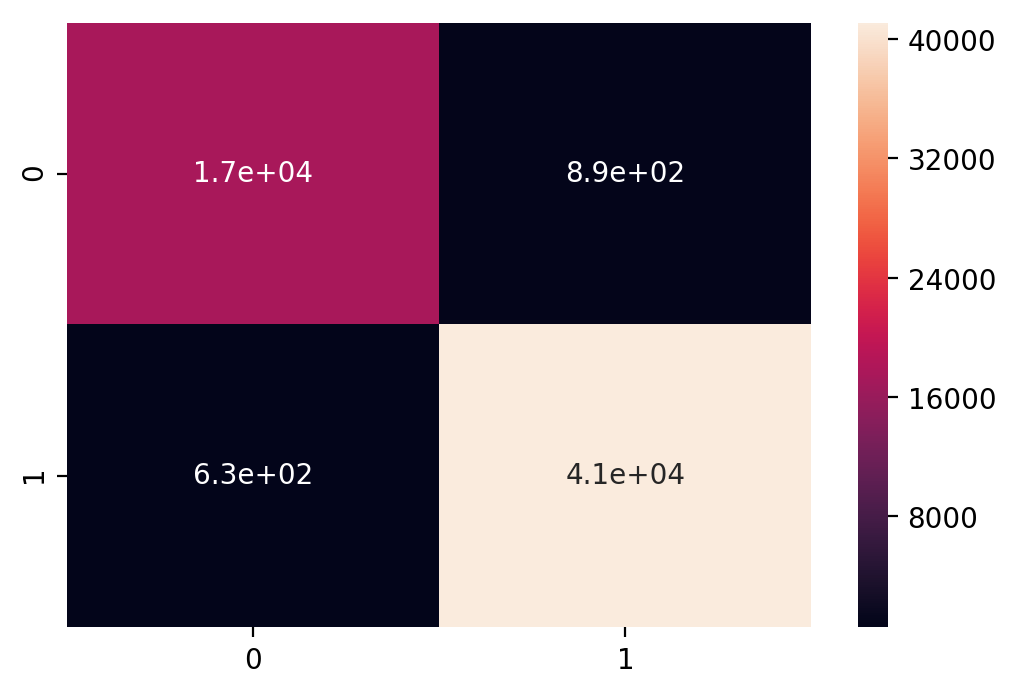
\includegraphics[width=0.32\textwidth]{./FigNSclass/CM_indRecCross}
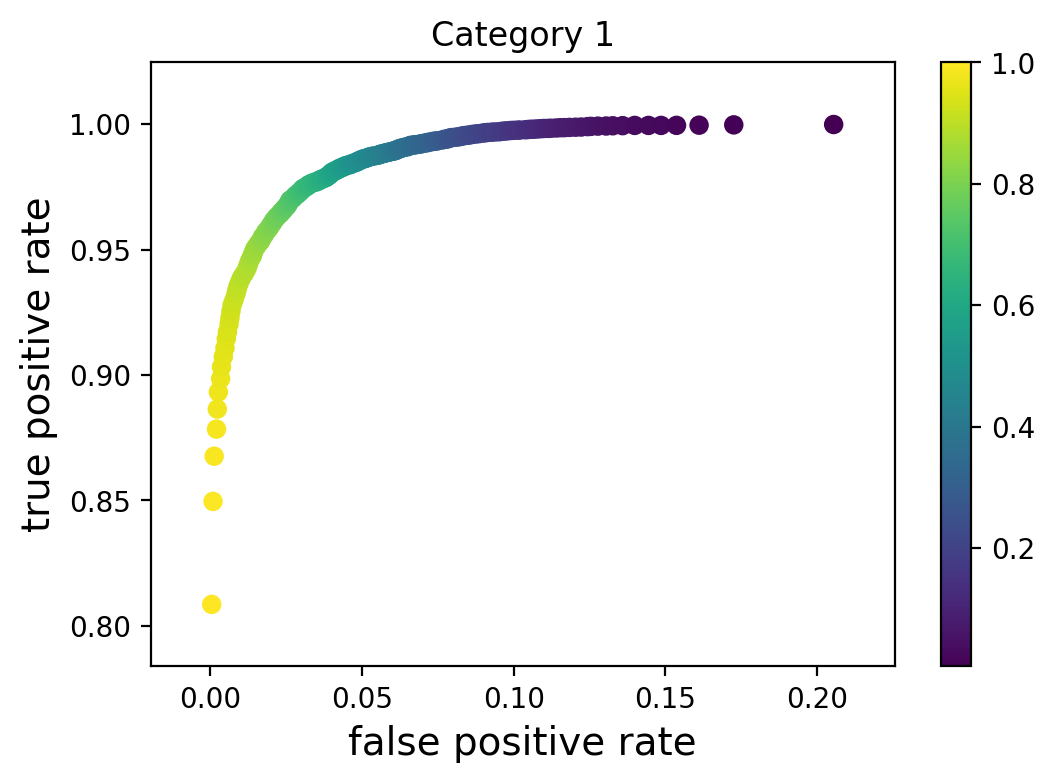
\includegraphics[width=0.32\textwidth]{./FigNSclass/rocCurve_indRecCross}
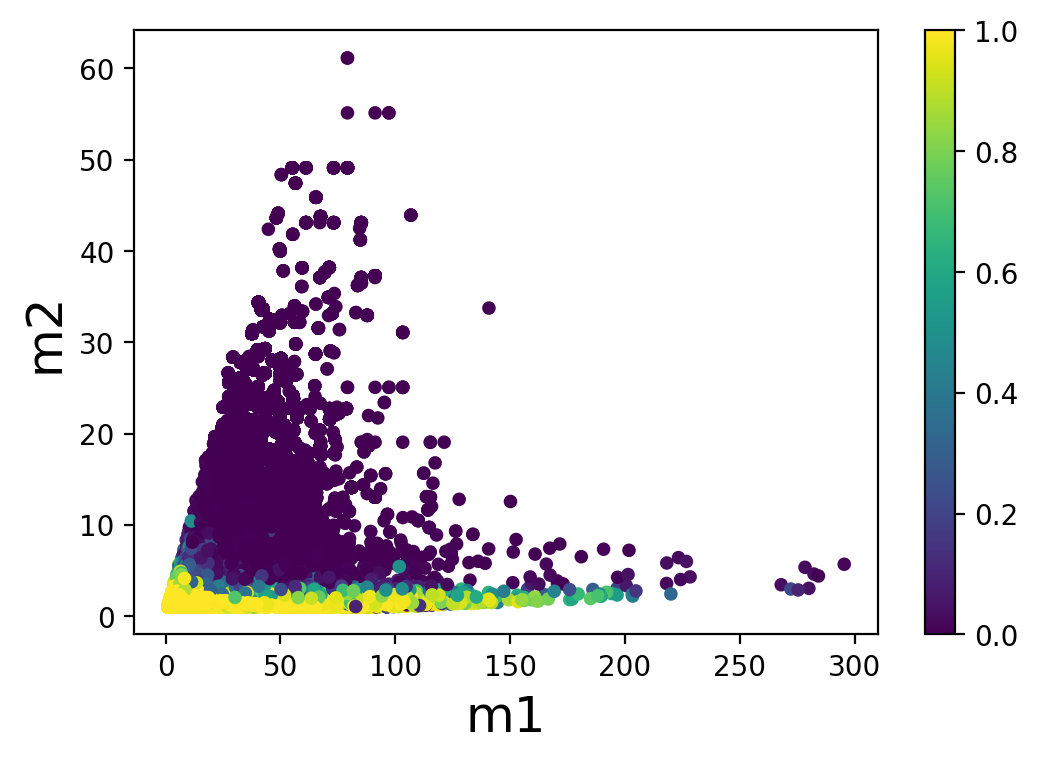
\includegraphics[width=0.32\textwidth]{./FigNSclass/scatterplot_indRecCross}
\caption{\label{fig:indreccross} Results with optimum model after crossvalidation. Using just independent recovered values (masses, spins and SNR).}
\end{figure}

\subsection{Using recovered variables}
Training and testing using: $m1_{rec}, m2_{rec}, chi1_{rec}, chi2_{rec}, mc_{rec}, q_{rec}, R_isco_{rec}, Compactness_{rec}, snr$.
Standard deviation of score during crossvalidation:  0.0002807499052054315 . Mean:  0.9744466574442907
Score  0.975032917215287 . Optimum forest found:  400  trees,  entropy  criteria and  sqrt  max features

Score on testing:  0.9745329088818147


\begin{figure}[]
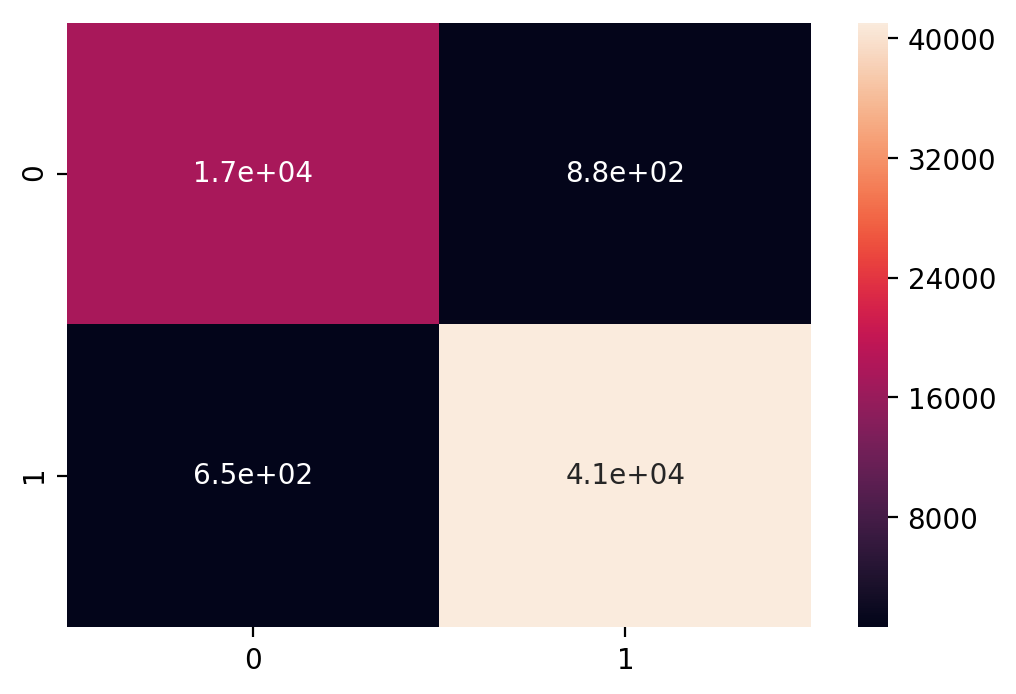
\includegraphics[width=0.32\textwidth]{./FigNSclass/CM_RecCross}
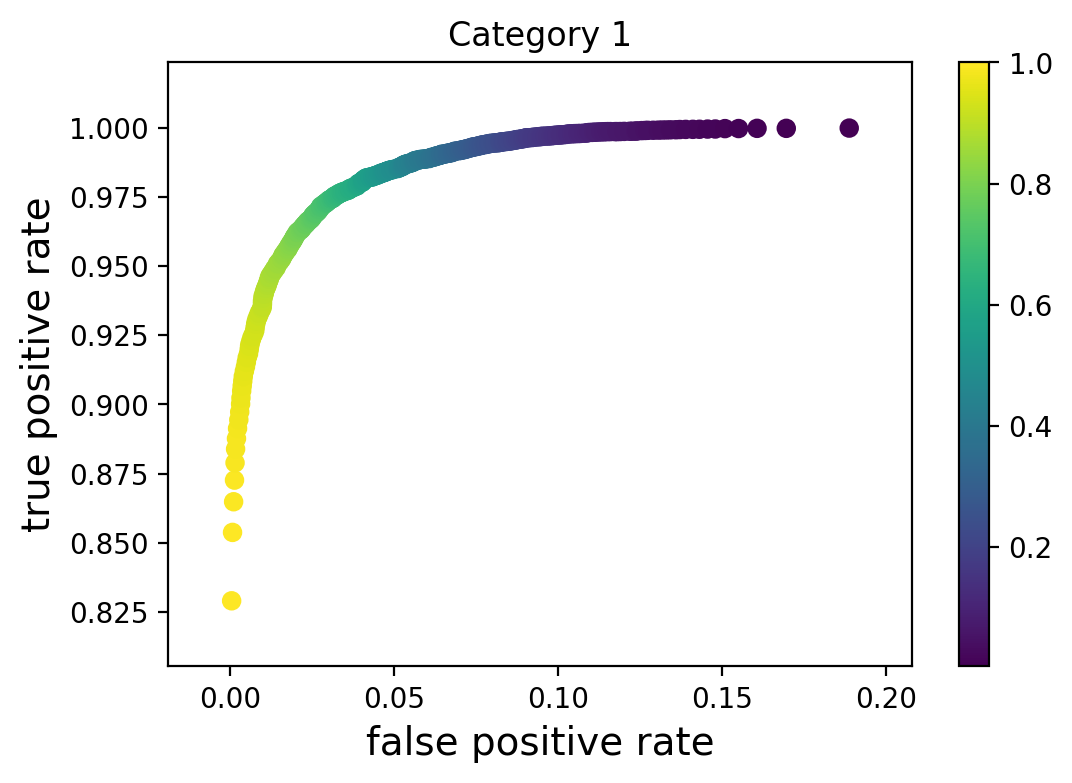
\includegraphics[width=0.32\textwidth]{./FigNSclass/rocCurve_RecCross}
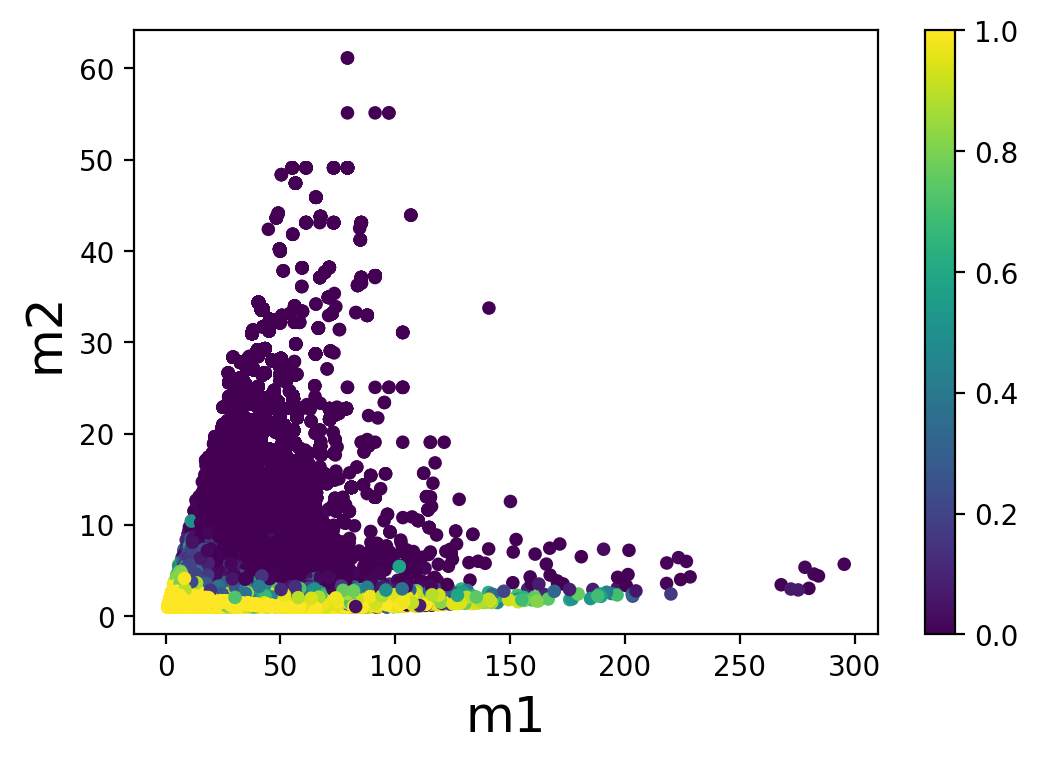
\includegraphics[width=0.32\textwidth]{./FigNSclass/scatterplot_RecCross}
\caption{\label{fig:indreccross} Results with optimum model after crossvalidation. Using all recovered values (masses, spins and SNR, mass ratio, chirp mass, compactness and Risco).}
\end{figure}

\subsection{All injected values}
No crossvalidated
Score on testing:  0.9999833330555509

\begin{figure}[]
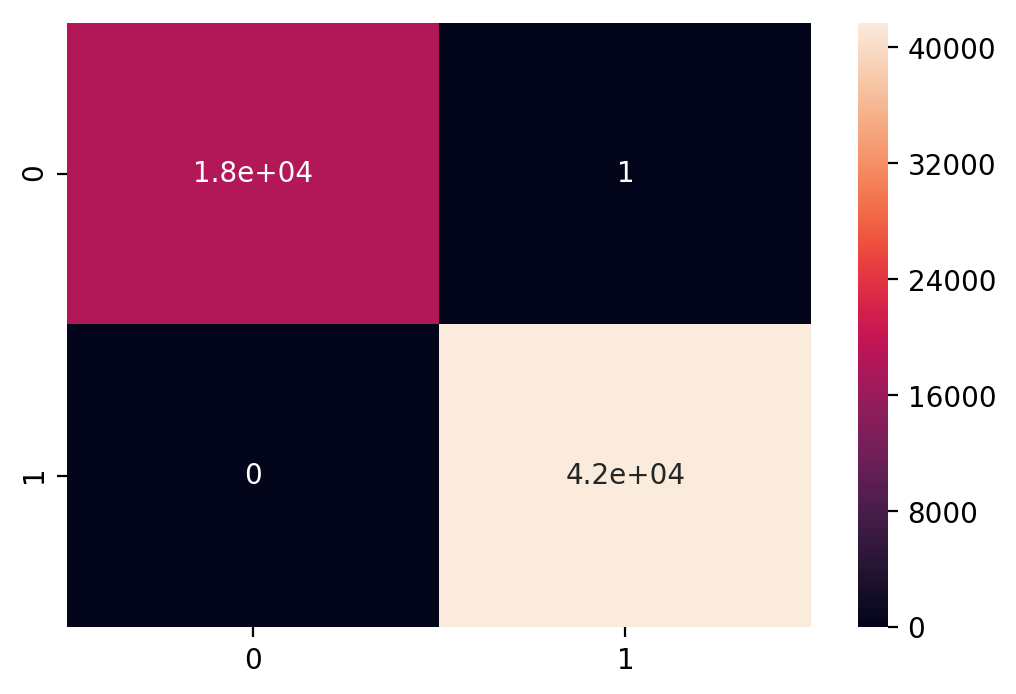
\includegraphics[width=0.32\textwidth]{./FigNSclass/CM_inj}
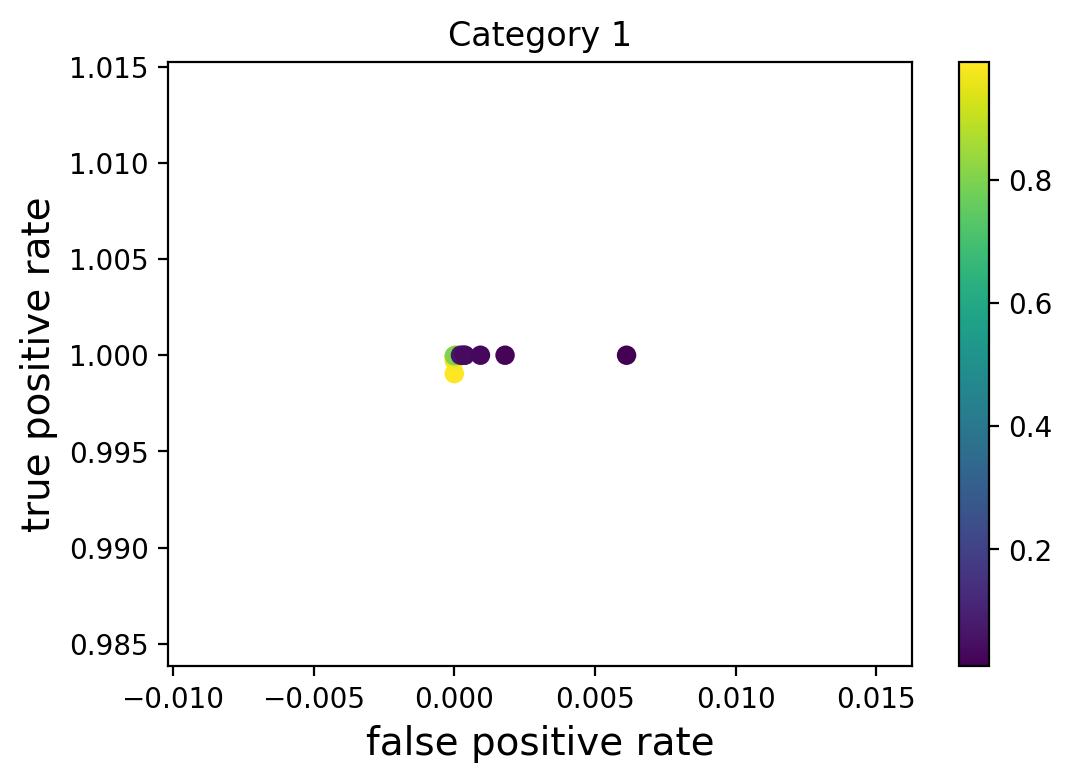
\includegraphics[width=0.32\textwidth]{./FigNSclass/rocCurve_inj}
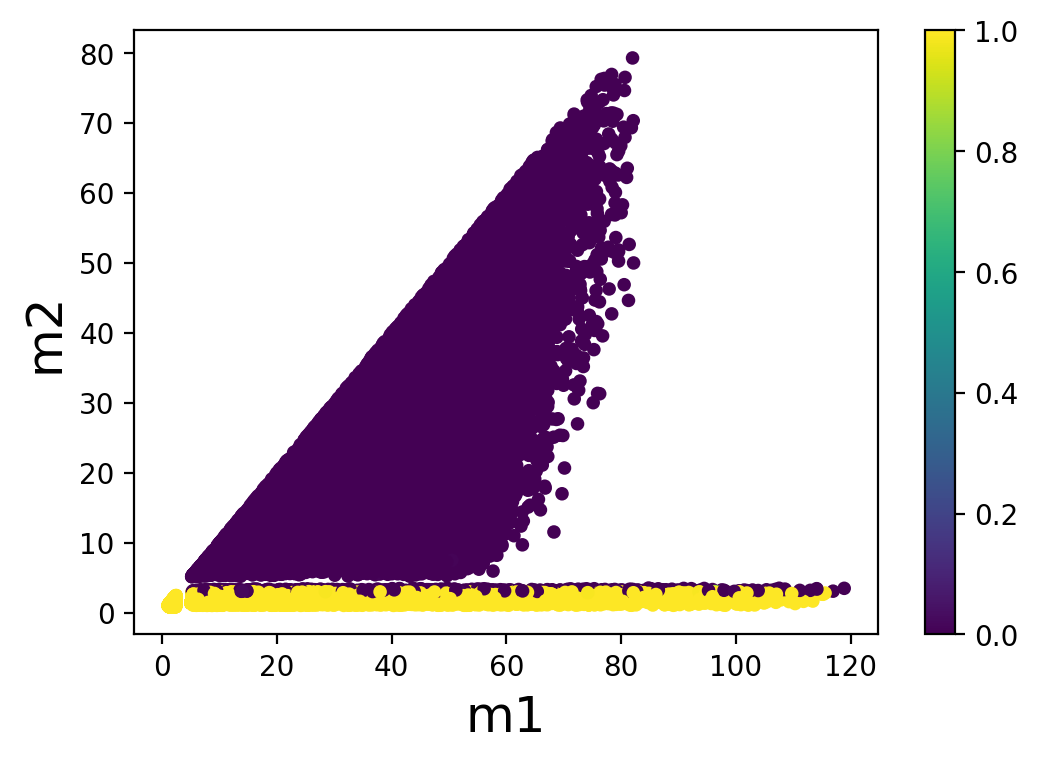
\includegraphics[width=0.32\textwidth]{./FigNSclass/scatterplot_inj}
\caption{\label{fig:inj} Results using all the injected values }
\end{figure}

\subsection{Independent injected values}
Score on testing:  0.9999833330555509

\begin{figure}[]
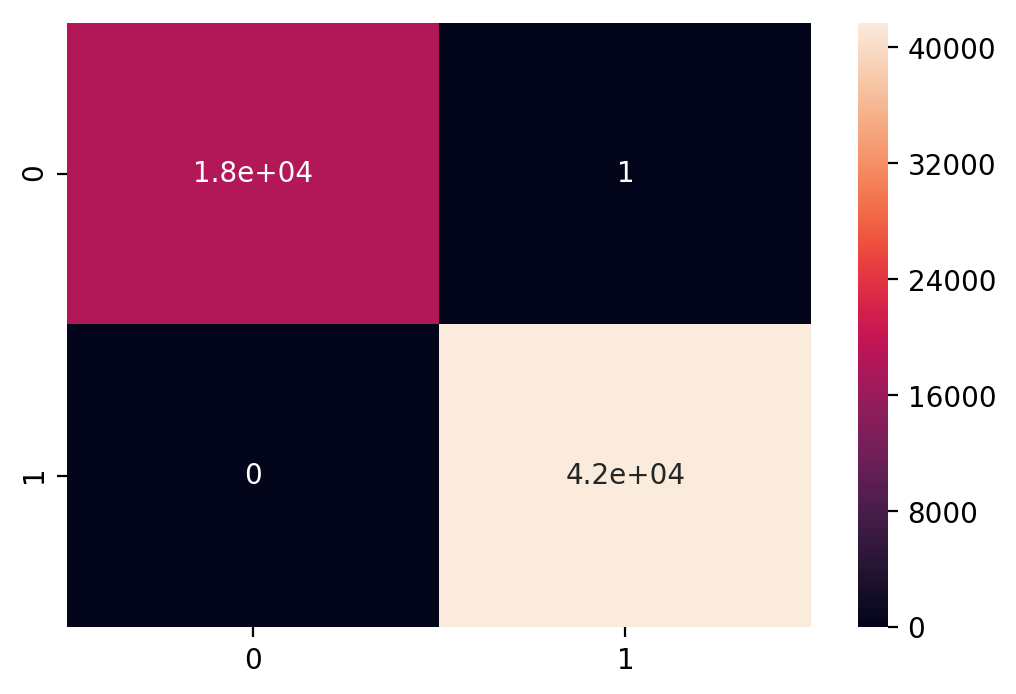
\includegraphics[width=0.32\textwidth]{./FigNSclass/CM_ind_inj}
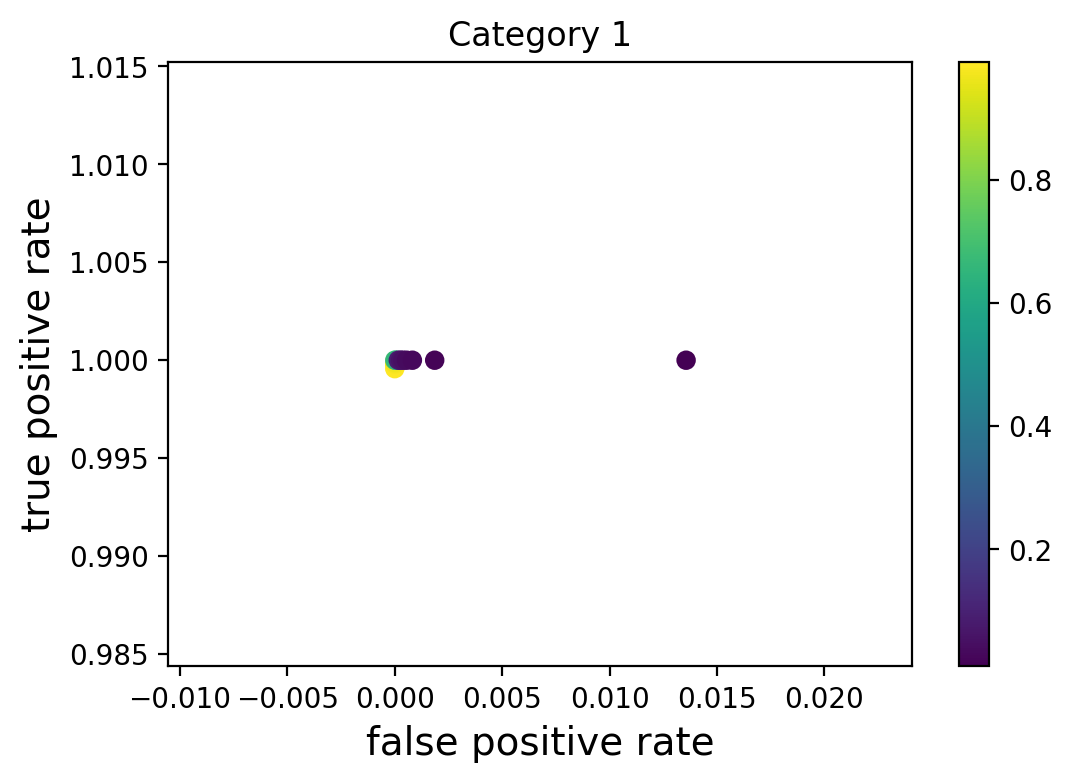
\includegraphics[width=0.32\textwidth]{./FigNSclass/rocCurve_ind_inj}
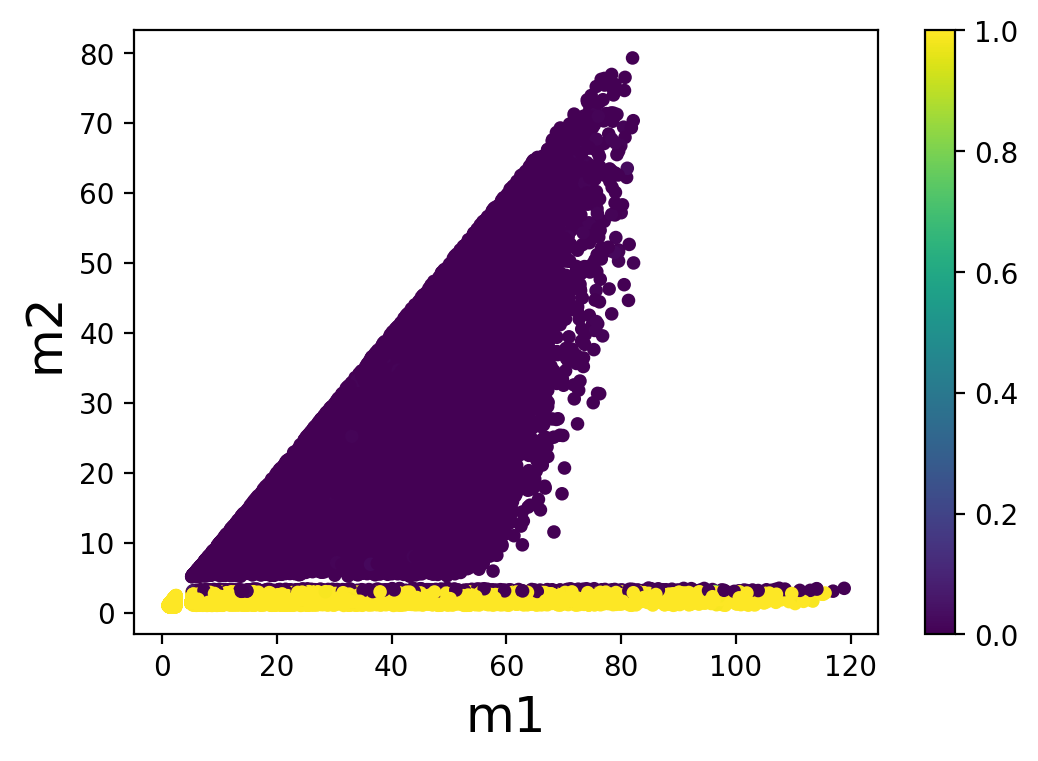
\includegraphics[width=0.32\textwidth]{./FigNSclass/scatterplot_ind_inj}
\caption{\label{fig:indinj} Results using the independent injected values}
\end{figure}

\end{document}